Eclipseも非常によく使われる開発ツールです。以下ではEclipseを使ってどのようにGoプログラムを編集するかご紹介します。

\begin{figure}[H]
  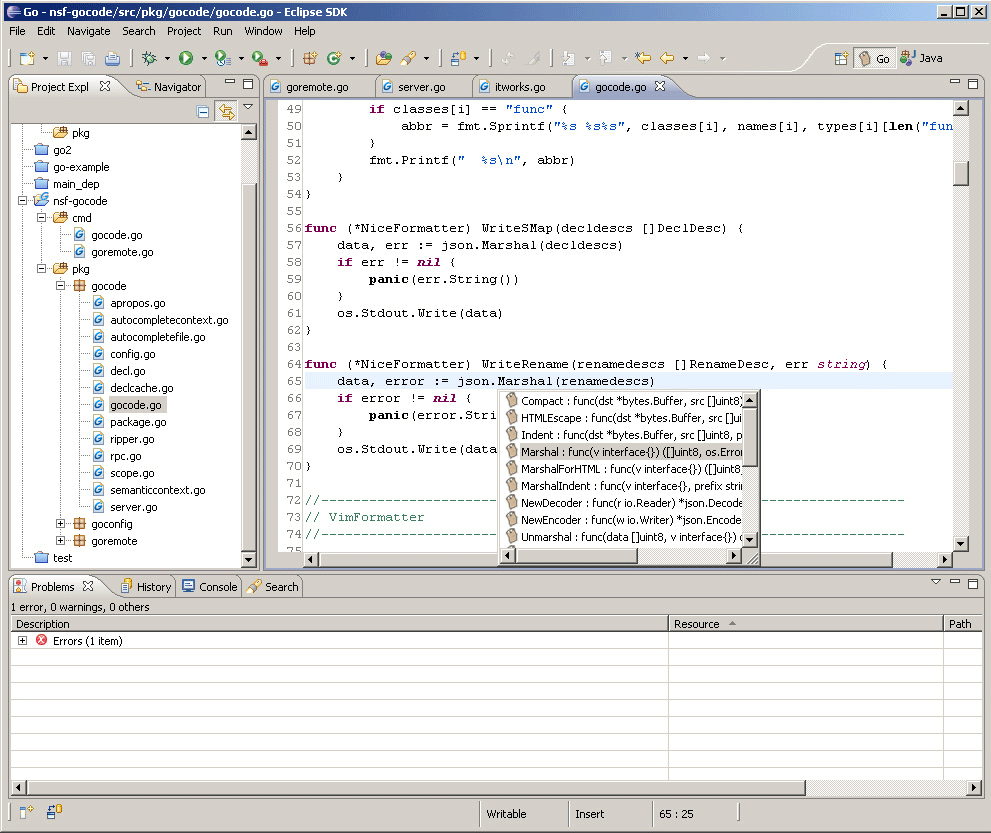
\includegraphics[width=14cm]{1.4.eclipse1.png}
   \label{図1.11}
   \caption{EclipseでのGo編集のメイン画面}
\end{figure}

\begin{enumerate}
\item まずEclipseをダウンロードしてインストールします。
\item goclipseプラグインをダウンロードします。\\ http:\//\//code.google.com\//p\//goclipse\//wiki\//InstallationInstructions
\item gocodeをダウンロードして、goのコード補完を表示させます。
\begin{lstlisting}[numbers=none]
 gocodeのgithubアドレス:
 https://github.com/nsf/gocode
 windowsではgitをインストールする必要があります。通常は
 [msysgit](https://code.google.com/p/msysgit/)を使います。
 cmdでインストールを行います:
 go get -u github.com/nsf/gocode
 以下のコードをダウンロードし、直接go buildでコンパイルしても
 かまいません。
 この場合はgocode.exeが生成されます。
\end{lstlisting}
\item MinGWをダウンロードして要求に従いインストールしてください。
\item プラグイン設定\\ Windows-$>$Reference-$>$Go
  \begin{enumerate}
  \item Goのコンパイラを設定します。
\begin{figure}[H]
  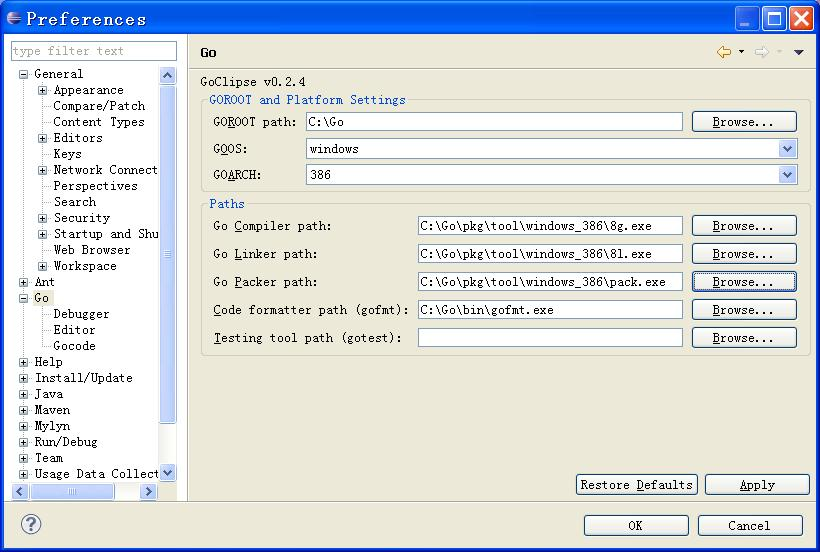
\includegraphics[width=14cm]{1.4.eclipse2.png}
   \label{図1.12}
   \caption{Goの基本情報を設定します。}
\end{figure}
  \item Gocodeを設定します(オプション、コード補完)、Gocodeのパスは事前に生成したgocode.exeファイルを設定します。
\begin{figure}[H]
  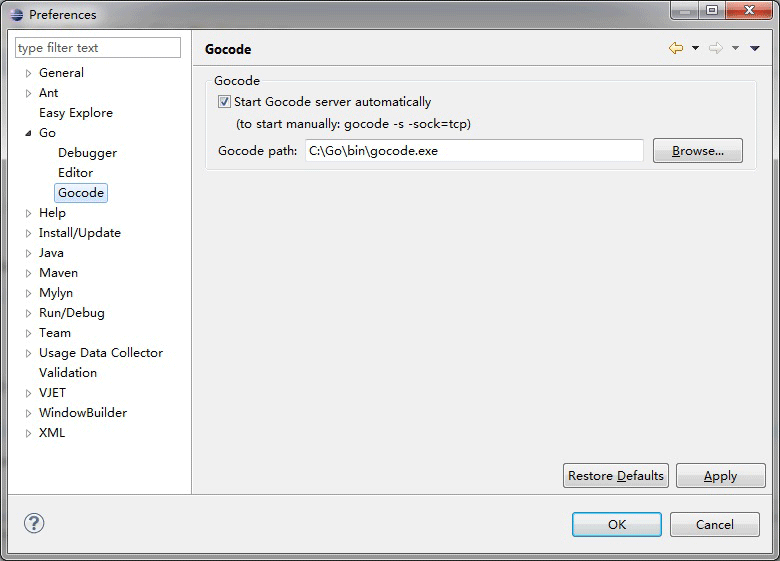
\includegraphics[width=14cm]{1.4.eclipse3.png}
   \label{図1.13}
   \caption{gocode情報を設定します。}
\end{figure}
  \item GDBを設定します(オプション、テスト用)、GDBのパスはMingGWのインストールディレクトリ下のgdb.exeファイルを設定します。
\begin{figure}[H]
  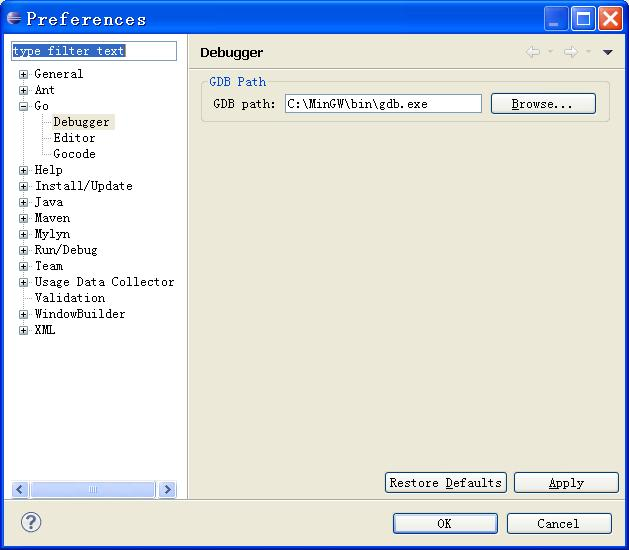
\includegraphics[width=14cm]{1.4.eclipse4.png}
   \label{図1.14}
   \caption{GDB情報の設定}
\end{figure}
  \end{enumerate}
\item テストが成功するか\\ goプロジェクトを一つ新規作成して、hello.goを作成します:
\begin{figure}[H]
   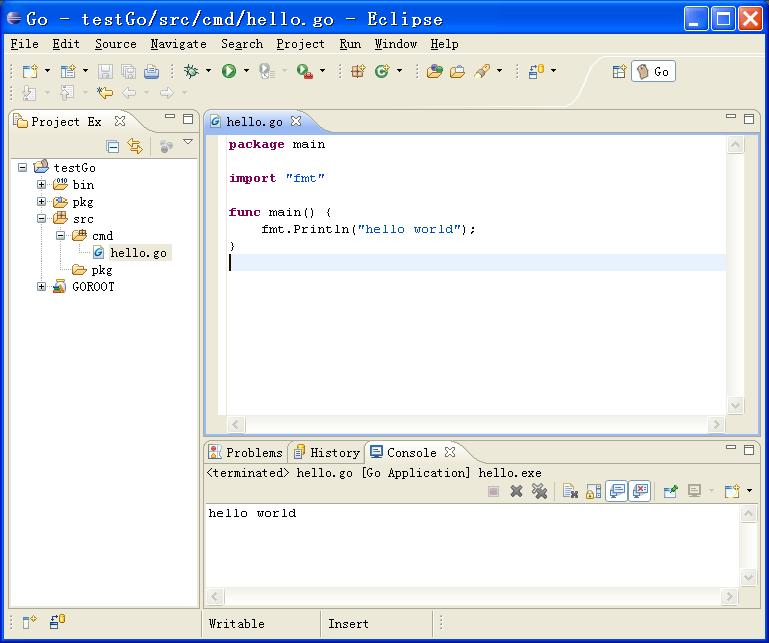
\includegraphics[width=14cm]{1.4.eclipse5.png}
   \label{図1
     .15}
   \caption{プロジェクトの新規作成とファイルの編集}
\end{figure}
\item テストの実行(consoleでコマンドを入力する必要があります):
\begin{figure}[H]
  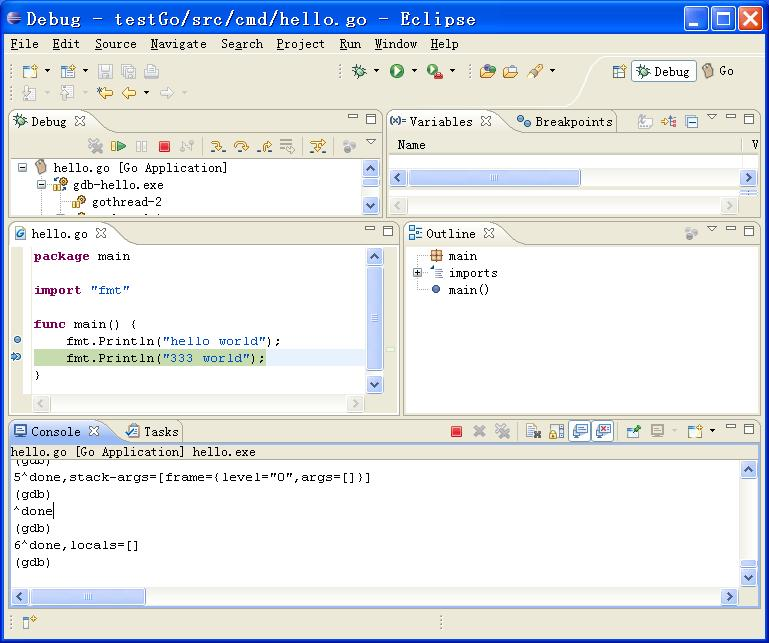
\includegraphics[width=14cm]{1.4.eclipse6.png}
   \label{図1.16}
   \caption{Goプログラムのテスト}
\end{figure}
\end{enumerate}
